\documentclass[12pt]{report}
\usepackage{../mystyle}
\begin{document}
\boldmath
\fancyhead[L]{Homework 1.}
\fancyhead[C]{Introduction to Knowledge Representation}
\fancyhead[R]{Ryabykin Aleksey}
    \begin{problem}{}
        Write in the existential graphs the following sentences:
        \begin{itemize}
            \item It's not true that it's raining and I didn't take the umbrella
            \item When it is raining, I take the umbrella
            \item Either it is not raining, or I took the umbrella
            \item If I did not take the umbrella, then it was not raining
            \item John and Bill are going to the movies, but not Tom 
            \item Susan doesn’t like squash or turnips
            \item If neither Peter nor Fred is going to the party, then neither will I
            \item If Mary hasn’t gotten lost or had an accident, she will be here in five minutes
        \end{itemize}
    \end{problem}
        \begin{figure}[H]
            \center
            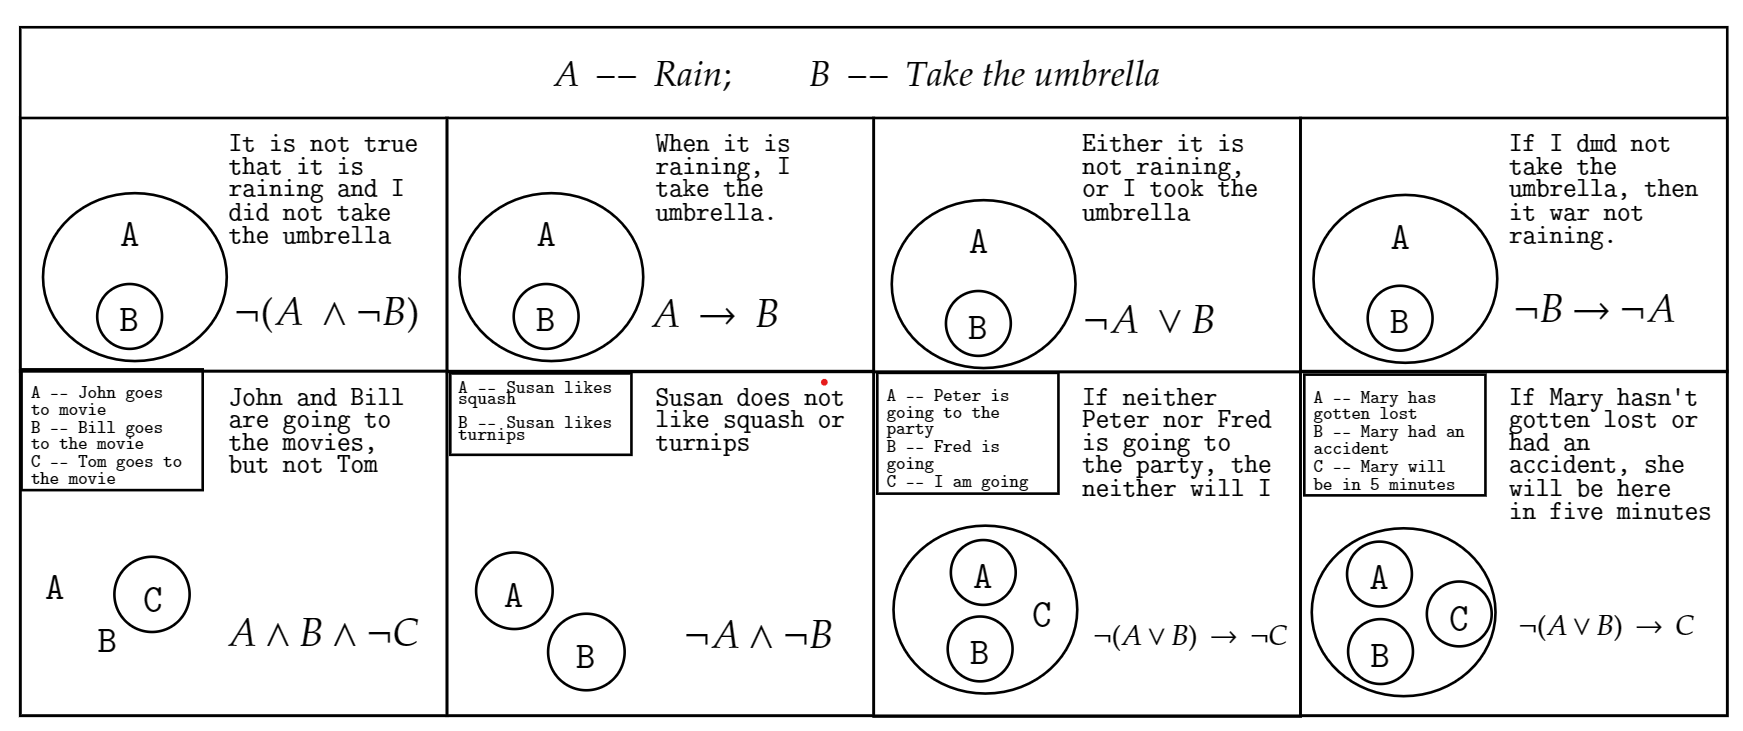
\includegraphics[scale=0.6]{p1.png}
        \end{figure}
    \begin{problem}{}
        Let A = John started the car, B = John pressed the gas pedal, C = The car started moving. 
        Read the following graph (that is, translate it into Russian) in at least three different ways:
    \end{problem}
    \begin{figure}[H]
        \center
        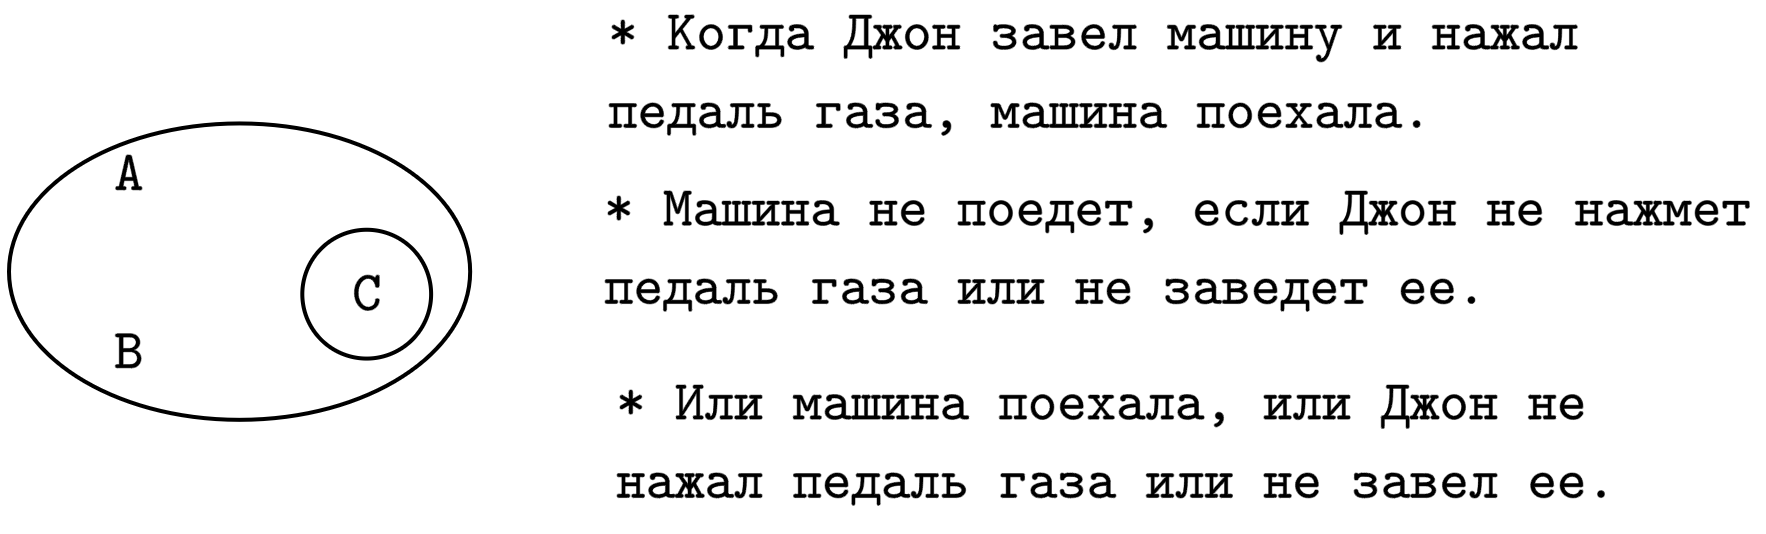
\includegraphics[scale=0.4]{p2.png}
    \end{figure}
    \begin{problem}{}
        \begin{enumerate}
        \item The butler or the cook or the chauffeur killed the baron. If the cook killed the baron, then the stew was poisoned, and if the chauffeur killed the baron, there was a bomb in the car. The stew wasn’t poisoned, and the butler didn’t kill the baron. Therefore, the chauffeur killed the baron.
        \item If the subject has not understood the instructions or has not finished reading the sentence, then he has pressed the wrong button or has failed to answer. If he has failed to answer, then the timer hasn’t stopped. The subject has pressed the right button, and the timer has stopped. Therefore, the subject understood the instructions.
        \end{enumerate}
    \end{problem}
    \begin{figure}[H]
        \center
        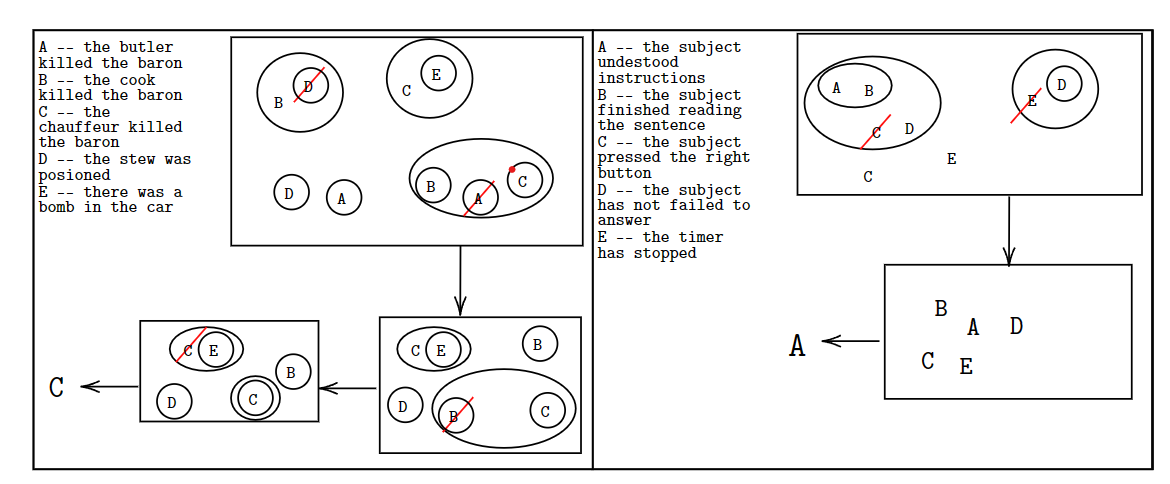
\includegraphics[scale=0.8]{p3.png}
    \end{figure}
    \begin{problem}{}
        Write in the existential graphs beta the following sentences
        \begin{enumerate}
        \item People who live in New York love it
        \item If John does not love New York, he does not live there (i. e. in it)
        \item If someone does not love New York, he does not know it
        \end{enumerate}
    \end{problem}
    \begin{figure}[H]
        \center
        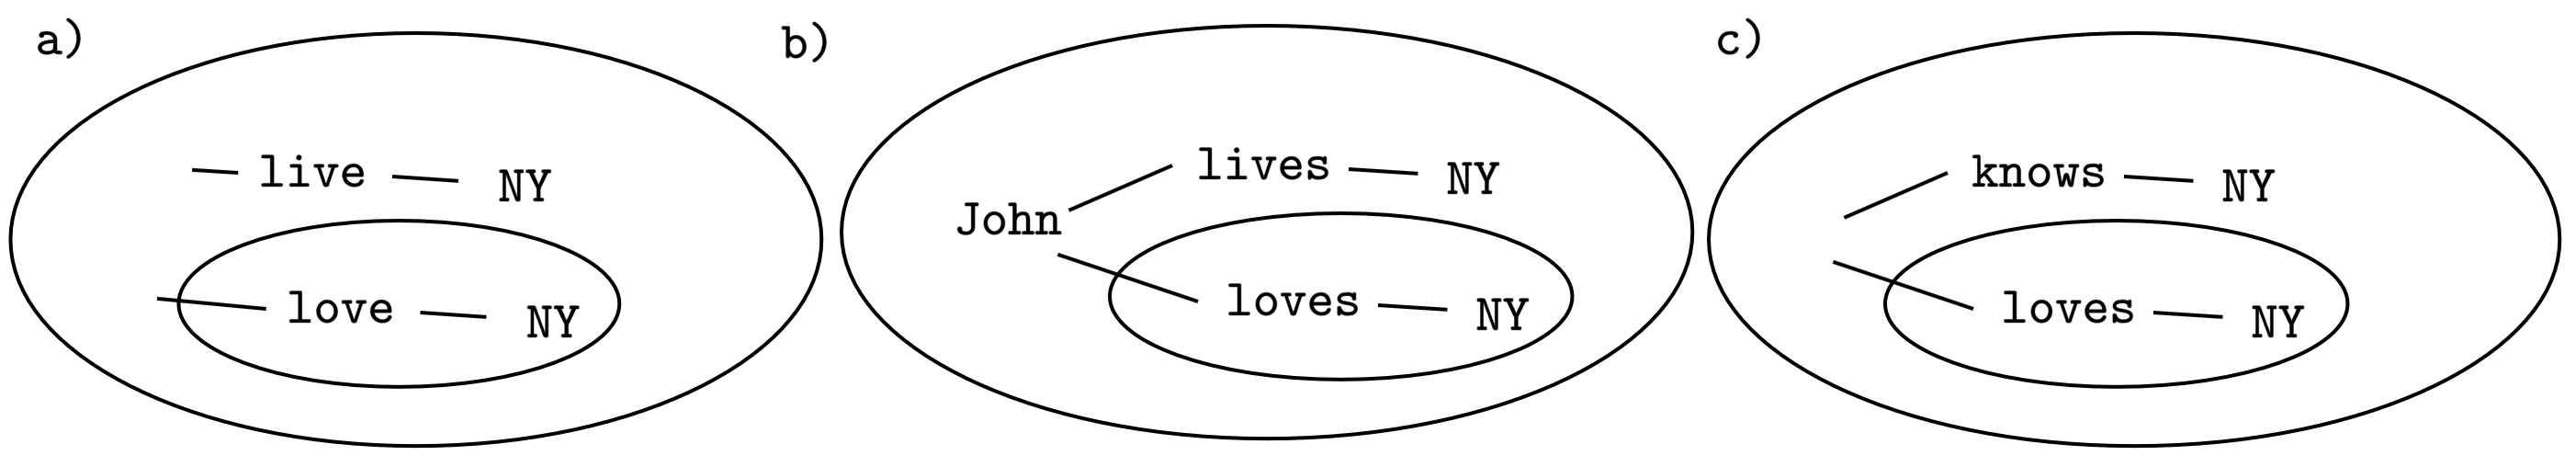
\includegraphics[scale=0.25]{p4.png}
    \end{figure}
    \begin{problem}{}

        \begin{enumerate}
            \item Babies are illogical. Nobody who is despised can manage a crocodile. Illogical persons are despised. Therefore, babies cannot manage crocodiles.
        \end{enumerate}
    \end{problem}
    Let's firstly construct the existential beta graph:
    \begin{figure}[H]
        \center
        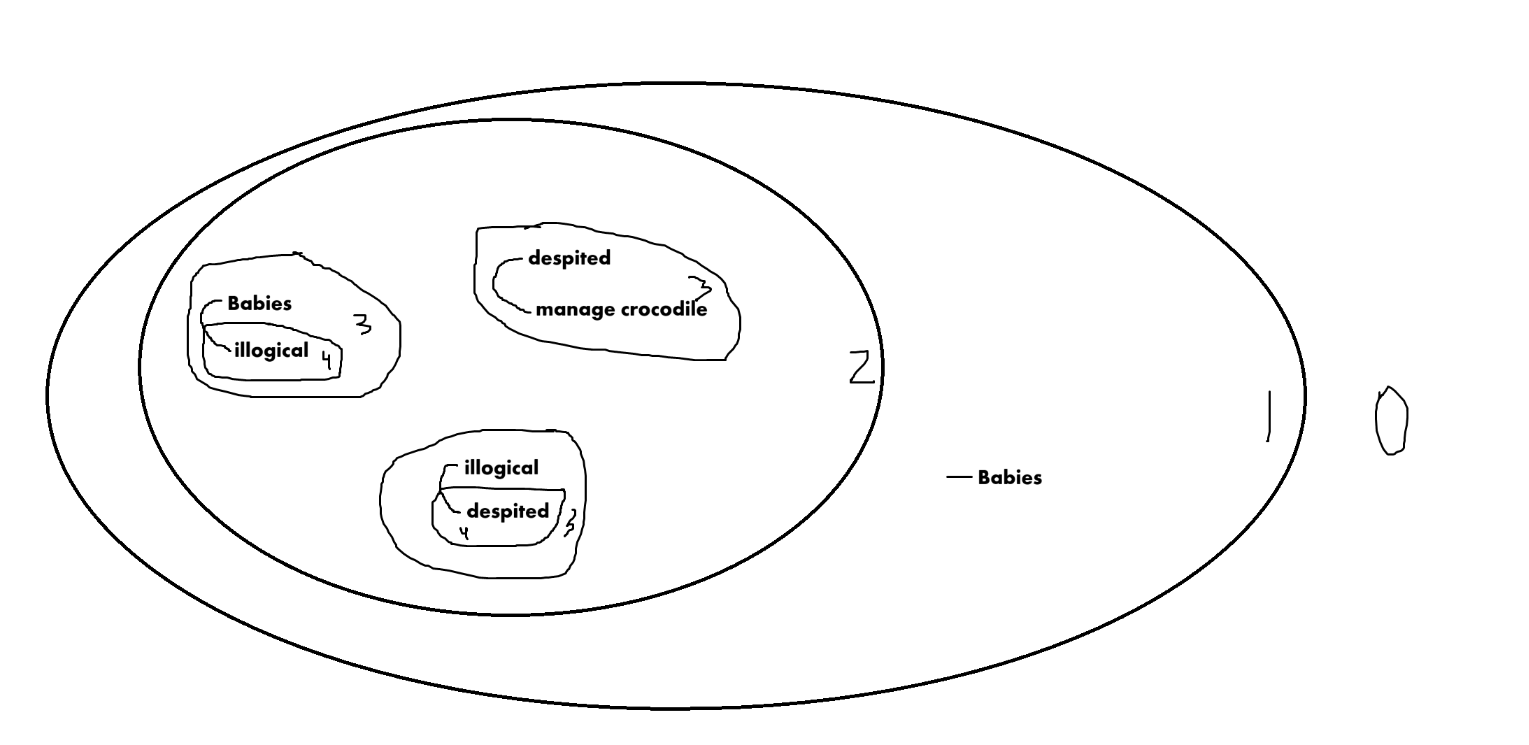
\includegraphics[scale=0.8]{p5a_1.png}
    \end{figure}
    To prove the implication we can to make double cut and add Babies into the first level. Then let's connect babies with Babies are illogical. Since we are on the odd level we connect lines and delete the copy babies:
    \begin{figure}[H]
        \center
        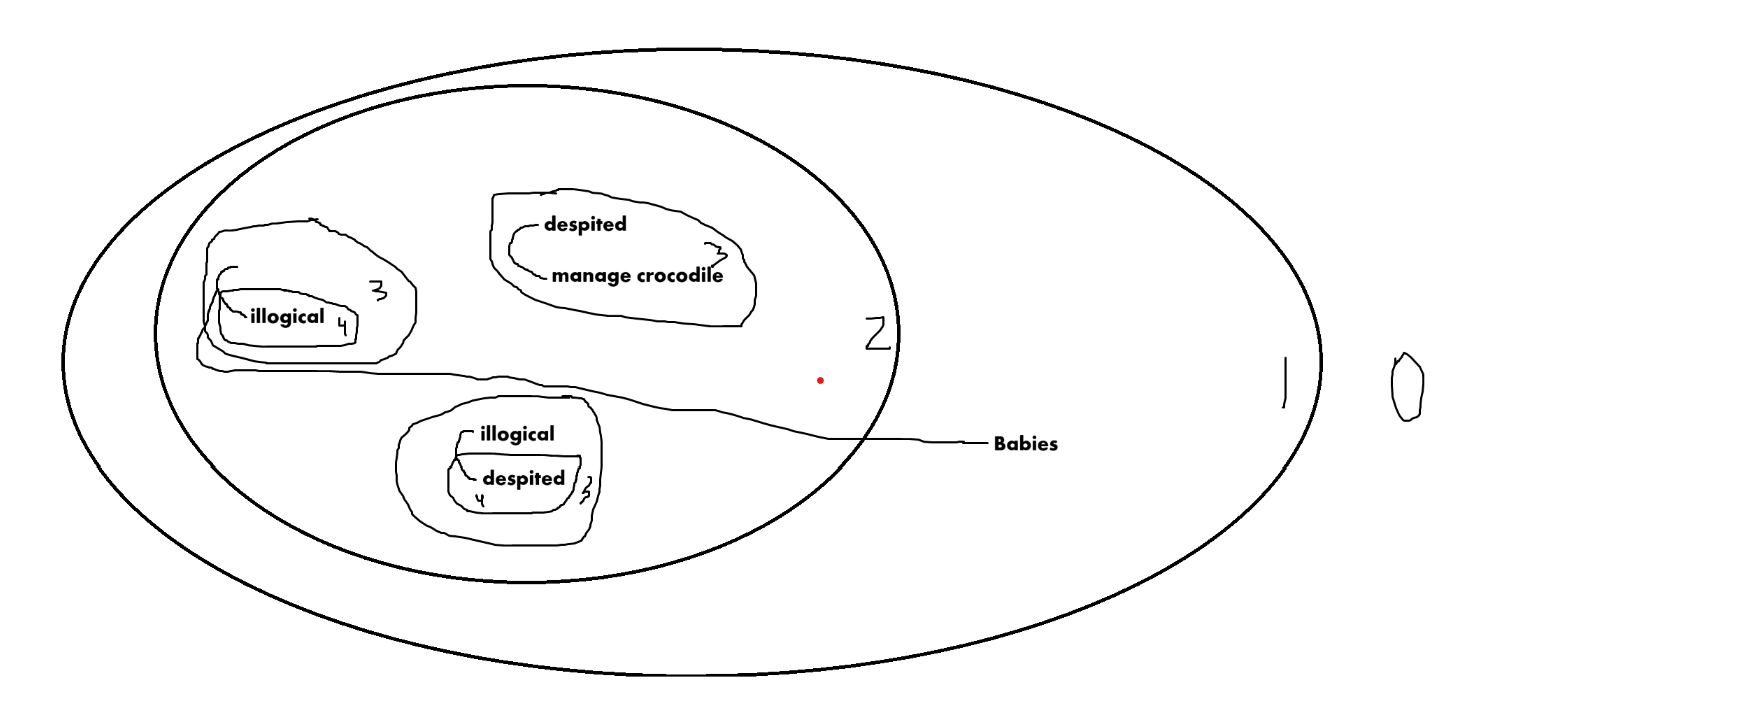
\includegraphics[scale=0.8]{p5a_2.png}
    \end{figure}
    Then we can reduce double negative. Add illogical into the illogical persons are despited, connect since the odd level and delete copy of illogical.
    \begin{figure}[H]
        \center
        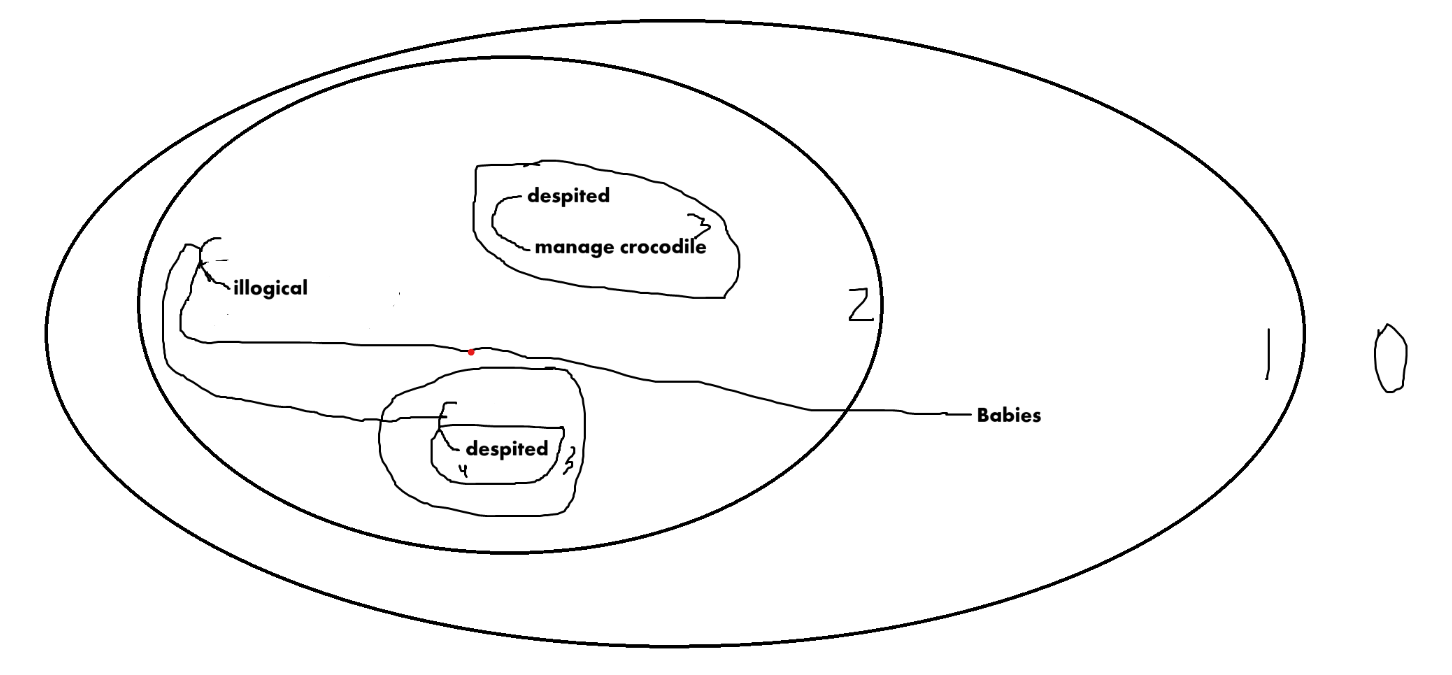
\includegraphics[scale=0.8]{p5a_3.png}
    \end{figure}
    Repeat same actions for despited and despited cannot manage crocodile. 
    \begin{figure}[H]
        \center
        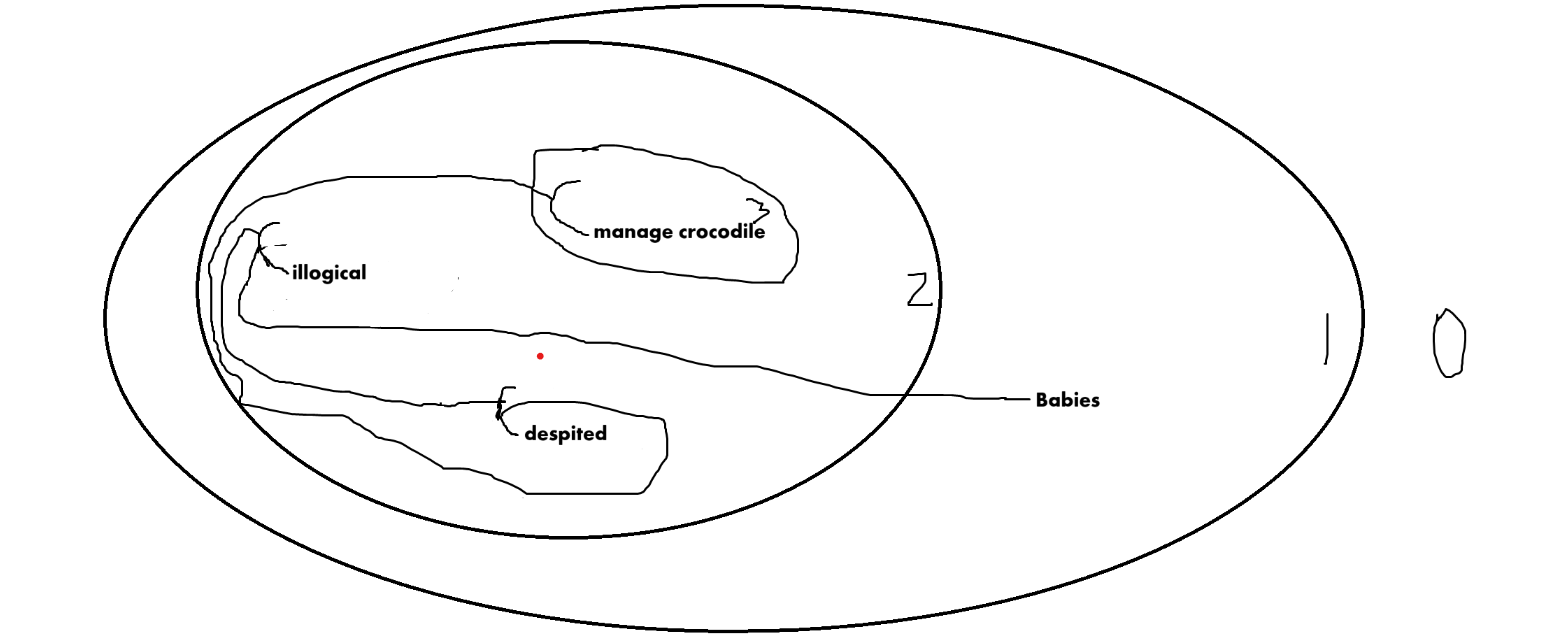
\includegraphics[scale=0.8]{p5a_4.png}
    \end{figure}
    On the even level we can erase any subgraph and reduce double negative. Hence we finally obtain:
    \begin{figure}[H]
        \center
        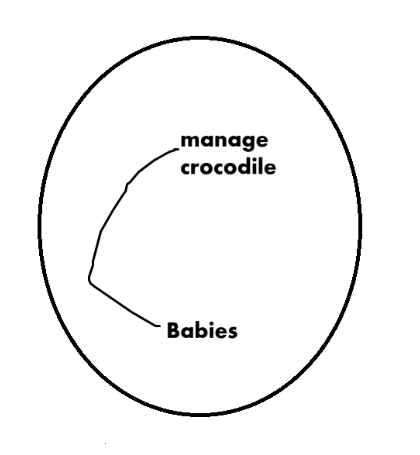
\includegraphics[scale=0.8]{p5a_5.png}
    \end{figure}

\end{document}
